\begin{figure}[p]\centering
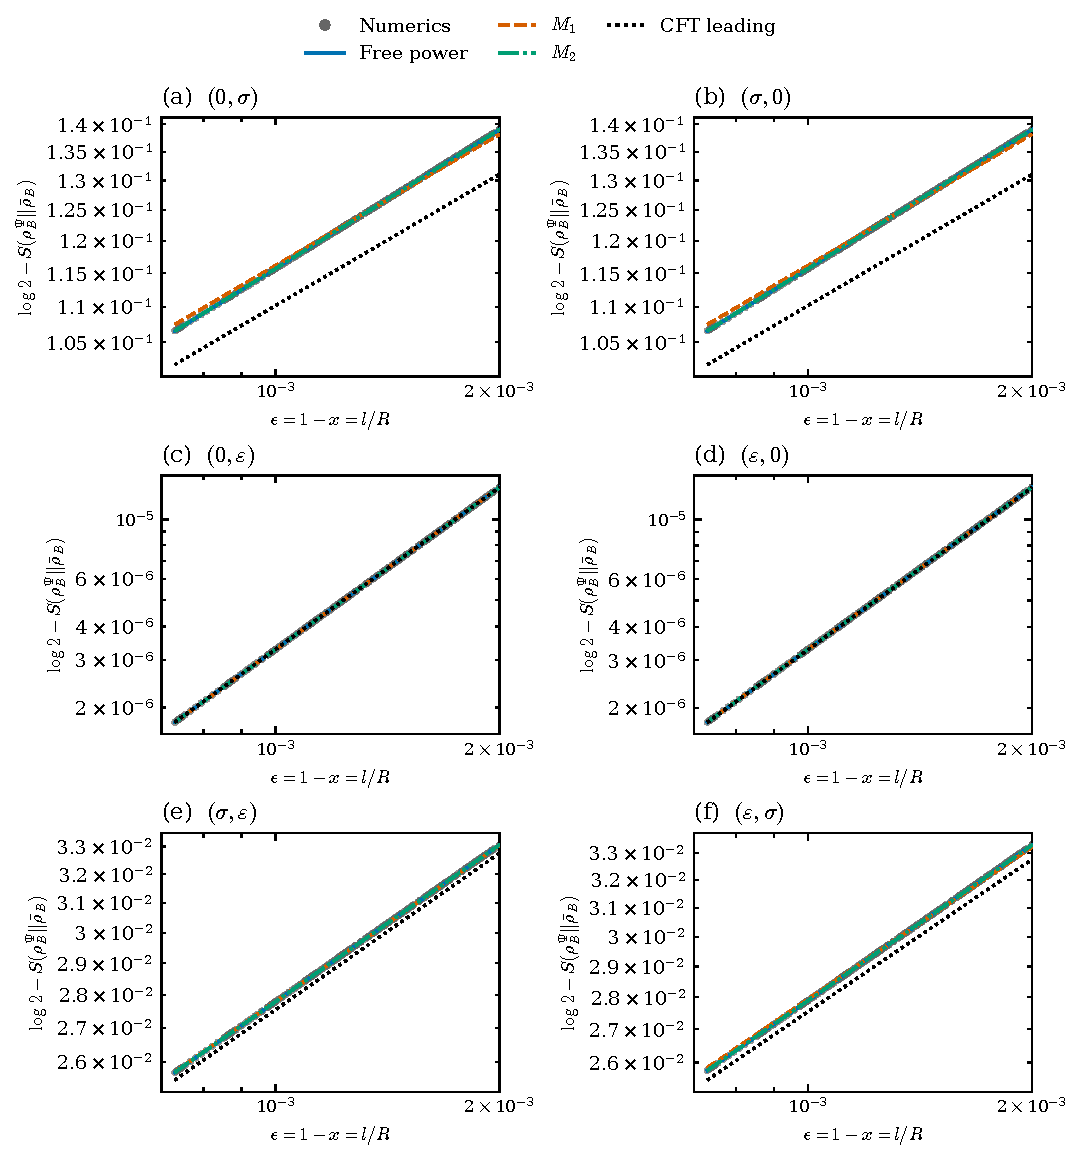
\includegraphics[width=.94\linewidth,height=.74\textheight,keepaspectratio]{figs/ising_large_fit_window_value.pdf}
\caption{Ising large-interval $\delta_{a\mid b}=\log2-D^B_{a\mid b}$ for all six ordered pairs. All 260 displayed geometries per direction lie in the fitting window $0<\ep\leq0.002$, with $\ell=6,\ldots,10$. Both axes are logarithmic. Gray circles denote numerical data, using the same shape and color for every subsystem length. Blue solid, orange dashed, and green dash--dotted curves denote the free fit, $F_1$, and $F_2$; black dotted denotes the parameter-free CFT leading term. All curves are restricted to the fitting window. The horizontal label $y$ denotes the complement fraction $\ep=1-x_B=\ell/N$, while the mixing probability is fixed at $1/2$.}
\label{fig:num-ising-large}
\end{figure}

\begin{figure}[p]\centering
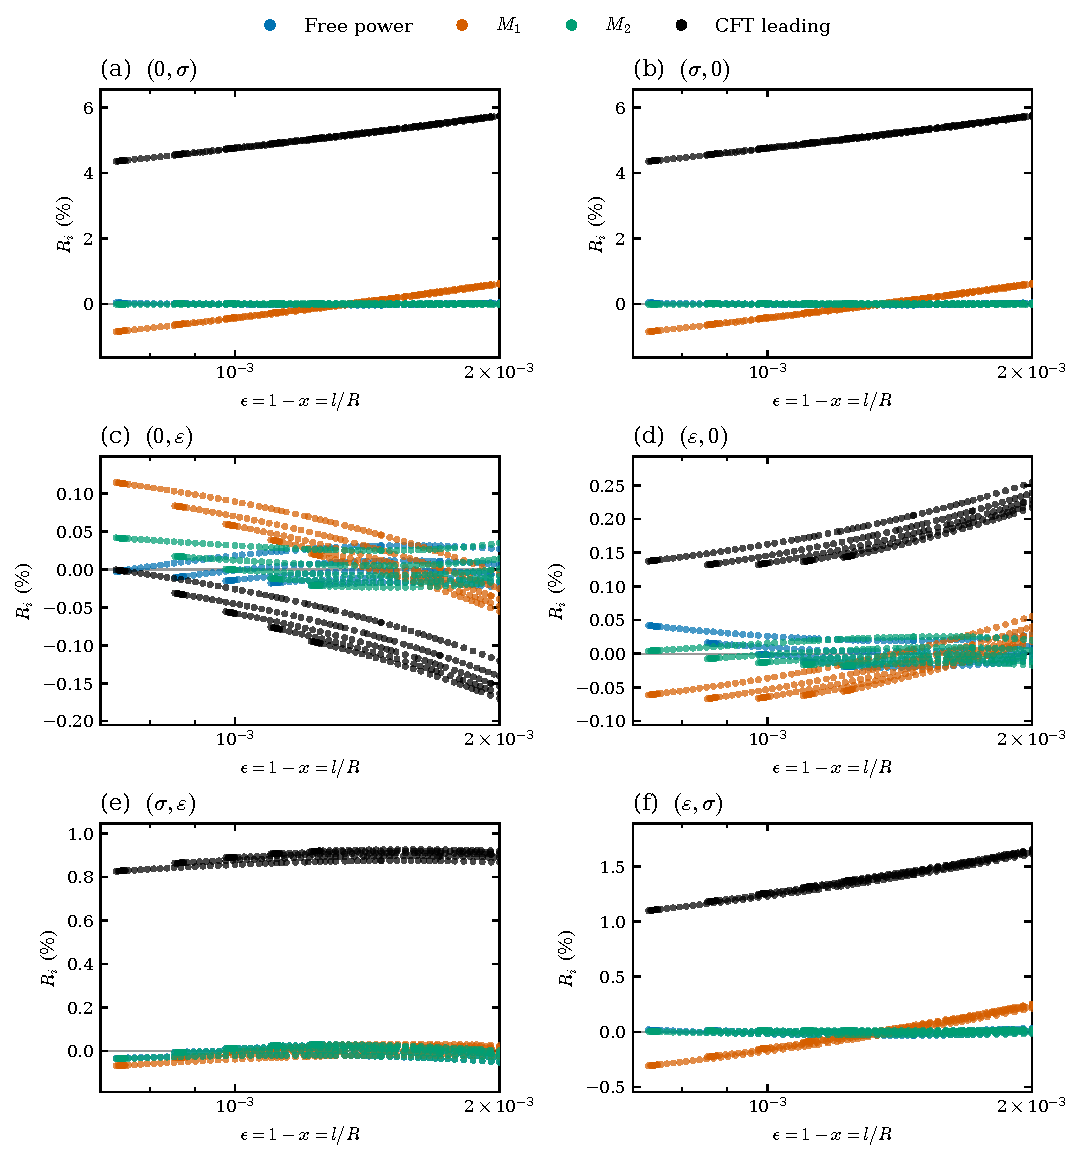
\includegraphics[width=.94\linewidth,height=.74\textheight,keepaspectratio]{figs/ising_large_fit_window_residual.pdf}
\caption{Signed percentage residuals $100[q-M]/q$ for Fig.~\ref{fig:num-ising-large}, with $q=\delta$. The residual ordinate is linear and the fraction axis logarithmic. Only the 260 fitted geometries per direction at $0<\ep\leq0.002$ are shown. All subsystem lengths $\ell=6,\ldots,10$ use circular markers; colors identify models and are identical across lengths. Blue, orange, green, and black denote the free fit, $F_1$, $F_2$, and the parameter-free CFT leading term. The horizontal label $y$ denotes the complement fraction $\ep=1-x_B=\ell/N$, while the mixing probability is fixed at $1/2$.}
\label{fig:num-ising-large-residual}
\end{figure}
